
\begin{figure}
	\centering
	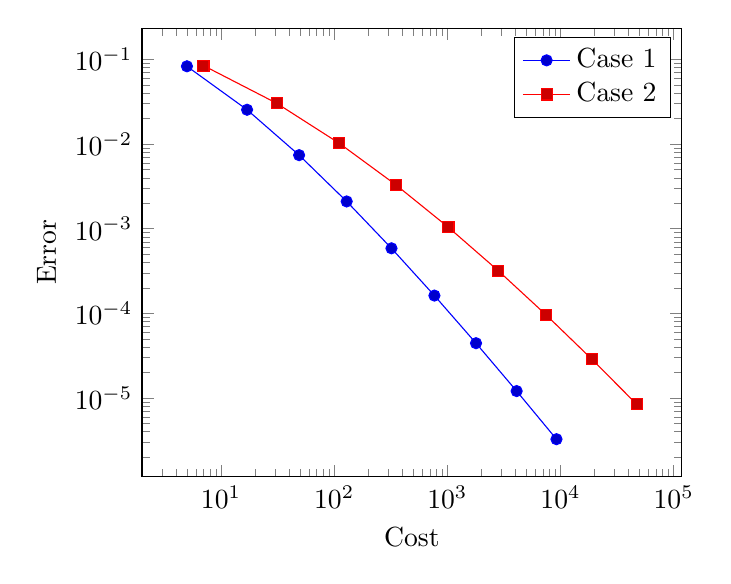
\begin{tikzpicture}
		\begin{loglogaxis}[
			xlabel=Cost,
			ylabel=Error]
		\addplot coordinates {
			(5,     8.31160034e-02)
			(17,    2.54685628e-02)
			(49,    7.40715288e-03)
			(129,   2.10192154e-03)
			(321,   5.87352989e-04)
			(769,   1.62269942e-04)
			(1793, 4.44248889e-05)
			(4097, 1.20714122e-05)
			(9217, 3.26101452e-06)
		};
		\addplot coordinates {
			(7,     8.47178381e-02)
			(31,    3.04409349e-02)
			(111,   1.02214539e-02)
			(351,   3.30346265e-03)
			(1023,  1.03886535e-03)
			(2815,  3.19646457e-04)
			(7423,  9.65789766e-05)
			(18943, 2.87339125e-05)
			(47103, 8.43749881e-06)
		};
		\legend{Case 1,Case 2}
		\end{loglogaxis}
	\end{tikzpicture}
	\caption{A larger example}
\end{figure}

\begin{figure}
\centering
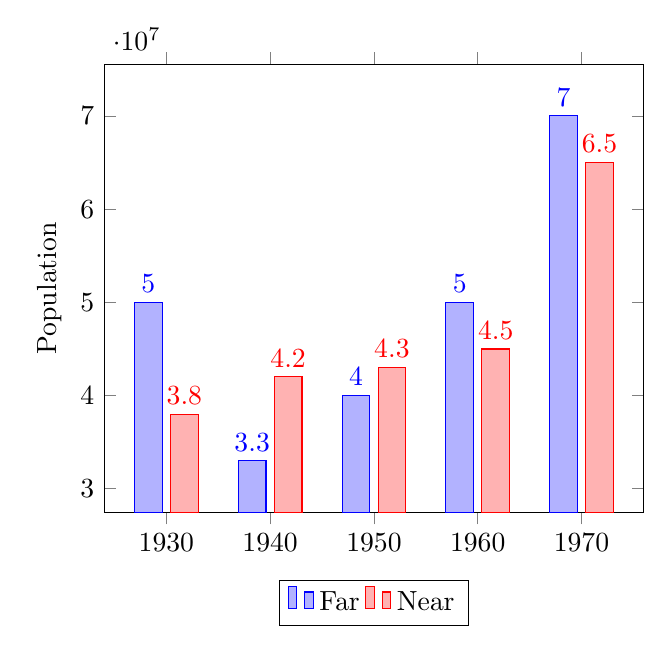
\begin{tikzpicture}
\begin{axis}[
	x tick label style={
		/pgf/number format/1000 sep=},
	ylabel=Population,
	enlargelimits=0.15,
	legend style={at={(0.5,-0.15)},
		anchor=north,legend columns=-1},
	ybar=3pt,% configures `bar shift'
	bar width=10pt,
	nodes near coords,
	point meta=y *10^-7 % the displayed number
]
\addplot 
	coordinates {(1930,50e6) (1940,33e6)
		 (1950,40e6) (1960,50e6) (1970,70e6)};

\addplot 
	coordinates {(1930,38e6) (1940,42e6) 
		(1950,43e6) (1960,45e6) (1970,65e6)};

\legend{Far,Near}
\end{axis}
\end{tikzpicture}
\caption{A double bar graph}
\end{figure}

\begin{figure}
\centering
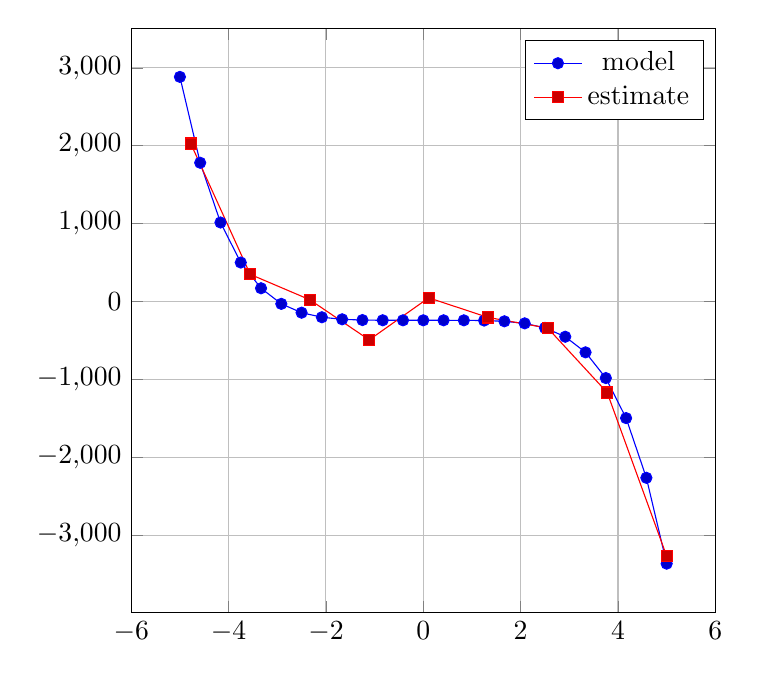
\begin{tikzpicture}
	\begin{axis}[
		height=9cm,
		width=9cm,
		grid=major,
	]
		
	\addplot {-x^5 - 242};
	\addlegendentry{model}

	\addplot coordinates {
		(-4.77778,2027.60977)
		(-3.55556,347.84069)
		(-2.33333,22.58953)
		(-1.11111,-493.50066)
		(0.11111,46.66082)
		(1.33333,-205.56286)
		(2.55556,-341.40638)
		(3.77778,-1169.24780)
		(5.00000,-3269.56775)
	};
	\addlegendentry{estimate}
	\end{axis}
\end{tikzpicture}
\caption{Inner Legend}
\end{figure}


\begin{figure}
\centering
\begin{tikzpicture}
	\begin{axis}[%
	scatter/classes={%
		a={mark=square*,blue},%
		b={mark=triangle*,red},%
		c={mark=o,draw=black}}]
	\addplot[scatter,only marks,%
		scatter src=explicit symbolic]%
	table[meta=label] {
x     y      label
0.1   0.15   a 
0.45  0.27   c 
0.02  0.17   a 
0.06  0.1    a 
0.9   0.5    b 
0.5   0.3    c 
0.85  0.52   b 
0.12  0.05   a 
0.73  0.45   b 
0.53  0.25   c 
0.76  0.5    b 
0.55  0.32   c
	};
	\end{axis}
\end{tikzpicture}
\caption{Clickable Coords}
\end{figure}


